%@Manual{,
%title = {R: A Language and Environment for Statistical Computing},
%author = {{R Development Core Team}},
%organization = {R Foundation for Statistical Computing},
%address = {Vienna, Austria},
%year = 2011,
%note = {{ISBN} 3-900051-07-0},
%url = {http://www.R-project.org}
%} 


%2multibyte Version: 5.50.0.2960 CodePage: 1252
%\documentclass[12pt]{article}%
\documentclass[11pt,oneside,fullpage]{amsart}
\usepackage{multirow}
\usepackage[top=1in, bottom=1in, left=1in, right=1in]{geometry}
\usepackage{booktabs}
\usepackage{dcolumn}
\usepackage{natbib}
\usepackage{graphicx}
\setcounter{MaxMatrixCols}{30}
\usepackage{amsfonts}
\usepackage{amsmath}
\usepackage{amssymb}
\usepackage{array,amsmath,graphicx,psfrag,amssymb,subfigure,tabularx,booktabs}
\usepackage{mparhack}
%\usepackage{listings}
%\lstset{language=R,basicstyle=\ttfamily}
\usepackage{tikz}
\tikzstyle{block} = [draw, fill=white, rectangle, 
    minimum height=3em, minimum width=6em]
\tikzset{>=stealth,pil/.style={->,thick,shorten <=2pt,shorten >=2pt,},
pil2/.style={<->,thick,shorten <=2pt,shorten >=2pt,}
}
\usetikzlibrary{positioning}
\usetikzlibrary{decorations.pathreplacing}
\usepackage{setspace}
\usepackage{multicol}
\usepackage{longtable}
\usepackage{hyperref}
\hypersetup{
    colorlinks=true,
    linkcolor=red,
    filecolor=cyan,      
    urlcolor=magenta,
    citecolor=blue,
    }
\usepackage{stmaryrd}
\setcitestyle{authordate,round,semicolon,aysep={,},yysep={,}}
\bibpunct[:]{(}{)}{;}{a}{,}{,}
%TCIDATA{OutputFilter=latex2.dll}
%TCIDATA{Version=5.50.0.2960}
%TCIDATA{Codepage=1252}
%TCIDATA{CSTFile=LaTeX article (bright).cst}
%TCIDATA{Created=Monday, June 04, 2012 18:16:39}
%TCIDATA{LastRevised=Sunday, June 17, 2012 15:55:14}
%TCIDATA{<META NAME="GraphicsSave" CONTENT="32">}
%TCIDATA{<META NAME="SaveForMode" CONTENT="1">}
%TCIDATA{BibliographyScheme=Manual}
%TCIDATA{<META NAME="DocumentShell" CONTENT="Standard LaTeX\Blank - Standard LaTeX Article">}
%TCIDATA{Language=American English}
%BeginMSIPreambleData
\providecommand{\U}[1]{\protect\rule{.1in}{.1in}}
%EndMSIPreambleData
\newtheorem{theorem}{Theorem}
\newtheorem{acknowledgement}[theorem]{Acknowledgement}
\newtheorem{algorithm}[theorem]{Algorithm}
\newtheorem{axiom}[theorem]{Axiom}
\newtheorem{case}[theorem]{Case}
\newtheorem{claim}[theorem]{Claim}
\newtheorem{conclusion}[theorem]{Conclusion}
\newtheorem{condition}[theorem]{Condition}
\newtheorem{conjecture}[theorem]{Conjecture}
\newtheorem{corollary}[theorem]{Corollary}
\newtheorem{criterion}[theorem]{Criterion}
\newtheorem{definition}[theorem]{Definition}
\newtheorem{example}[theorem]{Example}
\newtheorem{exercise}[theorem]{Exercise}
\newtheorem{lemma}[theorem]{Lemma}
\newtheorem{notation}[theorem]{Notation}
\newtheorem{problem}[theorem]{Problem}
\newtheorem{proposition}[theorem]{Proposition}
\newtheorem{remark}[theorem]{Remark}
\newtheorem{solution}[theorem]{Solution}
\newtheorem{summary}[theorem]{Summary}
%\newenvironment{proof}[1][Proof]{\noindent\textbf{#1.} }{\ \rule{0.5em}{0.5em}}
\usepackage{etoolbox}
\patchcmd{\subsection}{\bfseries}{\itshape \centering}{}{}
\patchcmd{\subsection}{-.5em}{.5em}{}{}

\begin{document}

\title[RebelTrack / RebelCast]{Introducing RebelTrack and RebelCast}
\thanks{This paper was prepared for the APSA 2017 Annual Meeting, August 30- September 3, San Francisco, CA. This is a preliminary draft. Please do not cite without contacting the authors. This research is funded by the Economic and Social Research Council (ES/L011506/1).}

%author two information
 

\author{Nils W. Metternich}
\address{Nils W. Metternich: Department of Political Science}
\curraddr{University College London, London, WC1H 9QU, UK}
\email{n.metternich@ucl.ac.uk}


\author{G{\"o}khan \c{C}\.{i}fl\.{i}kl\.{i}}
%\author{Gokhan Ciflikli}
\address{Gokhan Ciflikli: Department of International Relations}
\curraddr{London School of Economics and Political Science, London, WC2A 2AE, UK}
\email{g.ciflikli@lse.ac.uk}



\date{\today~~Version 1.03}
\maketitle

\begin{abstract}
This paper introduces RebelTrack (version 0.8), an R package leveraging mainly UCDP GED and PRIO GRID  datasets, which provides roughly 140 measures on rebel organization behavior. In addition, the paper introduces RebelCast a statistical learning framework to forecast rebel organization duration and escalation. The paper explains the main measures of RebelTrack and how this data is used in RebelCast to make predictions about rebel organization durations. We implement an ensemble learning approach to the prediction of rebel fighting durations that accommodates the unique challenges of duration data in this context. 
\end{abstract}

%\begin{abstract}
%Recent research provides strong support for the argument that rebel organization fragmentation increases fighting durations. However, not only rebel organizations, but also governments can be fragmented. From a bargaining perspective, we argue that ethnic fragmentation among, both, the government and rebel organizations increases the time to identify an agreement that satisfies all parties. In addition, the more economically diverse ethnic groups are within the government and the rebel organizations, the more pronounced this problem becomes as preferred redistribution ideal points differ. Bargaining situations where ethnic groups within the government and rebel organizations are economically very similar, multi-party bargaining collapses to 2-player situations and expected fighting times decrease. Using EPR data to identify which ethnic groups are part of the government and rebel organizations, we find empirical support for the hypothesis that government and rebel organizations with economically diverse ethnic groups (measured with night-light exposure data) fight longer armed conflicts.
%\end{abstract}

\onehalfspacing

\section{Introduction}
In the aftermath of the Arab Spring, the Syrian civil war started in 2011. Multiple rebel organizations have since been trying to oust the existing regime or claim considerable territories of the Syrian state and beyond. Five years later, the conflict is still ongoing, and it has claimed the life of up to half a million people. An estimated 12 million people left their homes, of which around four million crossed the Syrian border and became refugees. There is reason to believe that if the duration of fighting and the loss of lives would have been anticipated by the international community, we would have seen more effective strategies to end the conflict and more consolidated efforts to limit the number of people killed as a direct consequence of the longevity of the conflict. But could the duration of the Syrian war have been predicted \citep[e.g.][]{Pilster01072014} and why are not more researchers engaging in predicting the behavior (duration, escalation, termination) of rebel organizations. We believe that while much of the data exists to make predictions, the start-up costs in compiling data from multiple sources and `cleaning' them is high. Hence, we provide a RebelTrack a software package that provides functions to generate, aggregate, impute, and merge information on rebel organizations. We also think that many researchers perceive high costs in implementing prediction models. Thus, we provide a framework for predicting rebel organization duration and escalation that addresses fundamental issues in this domain, such as temporal and spatial dependence. 

In the civil war literature, we find very few examples of actually predicting civil war duration \citep{Pilster01072014,chiba:2015}.\footnote{\citet{mason1999win} represent a borderline case as they are interested in predicting the outcome of civil wars using duration models.} Most research on conflict duration focuses on explanatory approaches without considering the predictive power of models and variables. This limitation is quite surprising, as the field of conflict prediction is growing rapidly \citep[e.g.][]{gurr1986forecasting,o2002anticipating,schrodt2006forecasting,goldstone:2010,weidmann:2010,Schneider01022011,de2011new,ward2013,Gleditsch01012013,hegre2013predicting,bell2013coercion,brandt2014evaluating,Muchlinski01012016}. However, most predictive and forecasting models of civil war have focused on the onset and occurrence of conflict and less on the escalation, termination, and duration of fighting. 

In this paper, we provide a forecasting framework to the prediction of rebel fighting durations (RebelCast), which is based in data generated by RebelTrack. RebelTrack is a set of functions that generates measures of rebel activities based on the UCDP GED \citep{sundberg:2013} and PRIO-GRID dataset \citep{priogrid}. RebelTrack will be open for public development to create a large source of indicators for rebel organizations. RebelTrack is very much based on the idea that our discipline has invested too little in open software development to leverage existing data projects. While open access data projects have become the norm, there is very little cumulative efforts in how to most effectively make use of the data. RebelCast on the other hand provides a statistical learning approach to the prediction of conflict duration and contributes to the literature by providing an ensemble approach in this context. 

\section{Civil Conflict Duration}
In this paper we distinguish between explanatory approaches to civil conflict duration and predictive approaches. In the majority, explanatory approaches rest on hypotheses testing, where the researchers intend to demonstrate that it is unlikely that an effect found in a given sample would not be found in the whole population. According to some $p$-value threshold it is determined whether a significant relationship between two variables exist. Predictive approaches are more interested in overall model performance and whether the outcome is indeed well predicted. Predictive approaches are usually aware of the fact that $p$-values do not determine predictive power and that `non-significant' variables can greatly help predictive performance \citep{ward10}. 


\subsection{Explanatory approaches}
Explanatory approaches to conflict duration dominate the literature, and they have greatly contributed to our understanding of duration dynamics \citep{hegre2004duration}. Structural factors such as poverty \citep{collier04}, low state capacity \citep{Mason01121996,balch00,derouen04}, and resources \citep{buhaug2009geography} have been systematically linked to conflict duration. Theoretically, these structural conditions provide opportunity structures that prolong fighting \citep{collier04,fearon04,hironaka2009}.

More recently, civil war duration has been linked to rebel organization characteristics \citep{cunningham09} and the way they fight wars \citep{balcells2014does}. \citet{cunningham09} demonstrate that rebel organizations that are relatively strong and have legal political wings fight shorter civil wars. Rebel characteristics also determine the outcome of conflicts, where rebel organizations with territorial control are less likely to lose against the government \citep{cunningham09} and strong rebel organizations are more likely to engage in mediated conflict outcomes \citep{clayton2013relative} and power-sharing arrangements \citep{gent2011relative}. However, not only rebel strength, but also ethnicity \citep{montalvo2010ethnic} and especially linkages to ethnic groups impact civil war duration. In this context, \citet{jwnm:2012} demonstrate that rebel organizations recruiting from and operating on behalf of ethnic groups that are excluded from state power are more enduring. The role of ethnicity is also relevant in the shadow of externally enforced democratization, when rebel leaders of small ethnic groups have incentives to continue fighting \citep{nm:11}.

The link between interventions and conflict duration has not only been considered in the context of ethnic conflicts \citep{nm:11} but is generally seen as an important determinant of civil war duration. \citet{regan02} expects biased third-party interventions establishing parity between the belligerents to prolong wars, whereas interventions giving a clear advantage to one of the conflict parties should lead to shorter wars. Similarly, \citet{balch00} argue that biased interventions lead to shorter conflicts if they enable one party to succeed in the armed contest. Empirically, \citet{balch00} demonstrate that biased and neutral interventions prolong civil wars, while \citet{regan02} only finds neutral military interventions to be associated with longer conflicts. \citet{balch08} argue that third party interventions decrease the time until the supported group achieves military victory, while third-party interventions, on both the government and opposition sides, increase the time until a negotiated settlement. \citet{doyle06} and \citet{fortna08a} point out that interventions and especially UN interventions can provide reliable information to the parties and thereby decrease conflict continuation\footnote{In the context of mediations, \citet{kydd06} defines more precise conditions under which third-parties can resolve information problems.}. However, \citet{cunningham10} argues that military interventions can actually increase information problems and demonstrates that interventions prolong conflicts, while \citet{werner05} attributes this empirical pattern to powerful domestic actors that are unsatisfied with the terms of a settlement. In regard to UN interventions more specifically, \citet{derouen04} suggests that they increase the expected time needed for victories and decrease the time until a truce or treaty. 

One of the most robust findings in the civil war duration literature is that not only international \citep{balch00,regan02,balch08}, but especially domestic actor constellations impact fighting durations. Analyzing the consequences of multi-actor conflicts, \citet{cunningham06} provides a veto player framework in which ``more parties involved in conflict make civil wars more difficult to resolve through negotiation and therefore of longer duration'' \citep[875]{cunningham06}. Indeed, from a bargaining perspective it can be expected that more actors decrease the size of the acceptable bargaining range, increase information asymmetries, create last mover advantages, and give rise to expected power shifts that make agreements and termination of conflicts more difficult \citep{cunningham06,cunningham2011barriers}. However, not only the mere number of rebel organizations prolong conflict, but also alliance and splintering dynamics that characterize multi-actor conflicts \citep{bakke:2012,bapat:2012,Fjelde2012,cunninghamK:2012}. For example, \citet{Christia2012} argues that rebel alliances fall apart and conflict endures, when already small power-shifts lead to changes in the hierarchy of power relationships. This argument is in line with \citet{akcinaroglu:2012}, who provides insights that credible alliances increase the chances of rebel victories. From a computation perspective \citet{findley:2012} demonstrate that fragmentation of rebel organizations might actually decrease fighting durations, very much in contrast to insights from \citet{cunningham06}. 

%\subsection{Predictive approaches}
%\citet{chiba:2015}
%\citet{Pilster01072014}
%Nils/Goekhan

\section{The role of actor characteristics and configurations}
Actor characteristics and configurations have been theoretically identified as important contributors to conflict duration \citep[e.g.][]{cunningham06,cunningham09,Christia2012}. Multiple actors on the rebel side are frequently linked to more difficult bargaining situations and longer war durations. The idea of rebel organizations as veto players implies suggests that the bargaining range shrinks with increasing numbers of actors \citep{cunningham06}, which magnifies incomplete information \citep{slantchev2004initiators} and commitment problems usually associated to long civil war durations \citep{fearon04}.  Multi-actor setting also give rise to alliance and fragmentation dynamics \citep{bakke:2012,bapat:2012,Fjelde2012,cunninghamK:2012}, which are argued to be associated with longer civil conflict duration \citep{Christia2012}.

Beyond rebel organization configurations, actor and dyadic characteristics are argued to be associated with the duration of civil conflicts. \citet{cunningham09} argue that stronger rebels fight shorter wars as they can gain quick concessions from the government. Their argument is slightly different from bargaining approaches that would anticipate that power parity (frequently linked to incomplete information \citep{reed:2003}) or expected power-shifts (commitment problems \citep{powell06}) increase the duration of conflicts. \citet{greig2015rebels} demonstrates that rebels that are able to operate closer to the capital are more likely to be granted peace negotiations. Similarly, successful terrorist attacks by rebel organizations \citep{thomas:2014} are also linked to the onset of peace negotiations.  This suggests that observable behavior of rebel organizations is linked to conflict dynamics and outcomes. 

%Much of the current literature on civil war duration focuses on active rebel organizations \citep{cunningham09} or ethnic groups that are actually linked to rebels \citep{jwnm:2012}. However, \citet{walter2009reputation} suggests that also dormant rebels or groups that could potentially align themselves with armed organizations impact on civil war dynamics. \citet{walter2009reputation} provides a reputation cost argument, which implies that governments are willing to pay and inflict high costs on challengers to manipulate the expected utility of potential challengers. Hence, an increase in potential challengers should be associated with governments willing to fight longer wars to increase the expected costs of entering a conflict with the state.

\begin{figure}
\raggedright
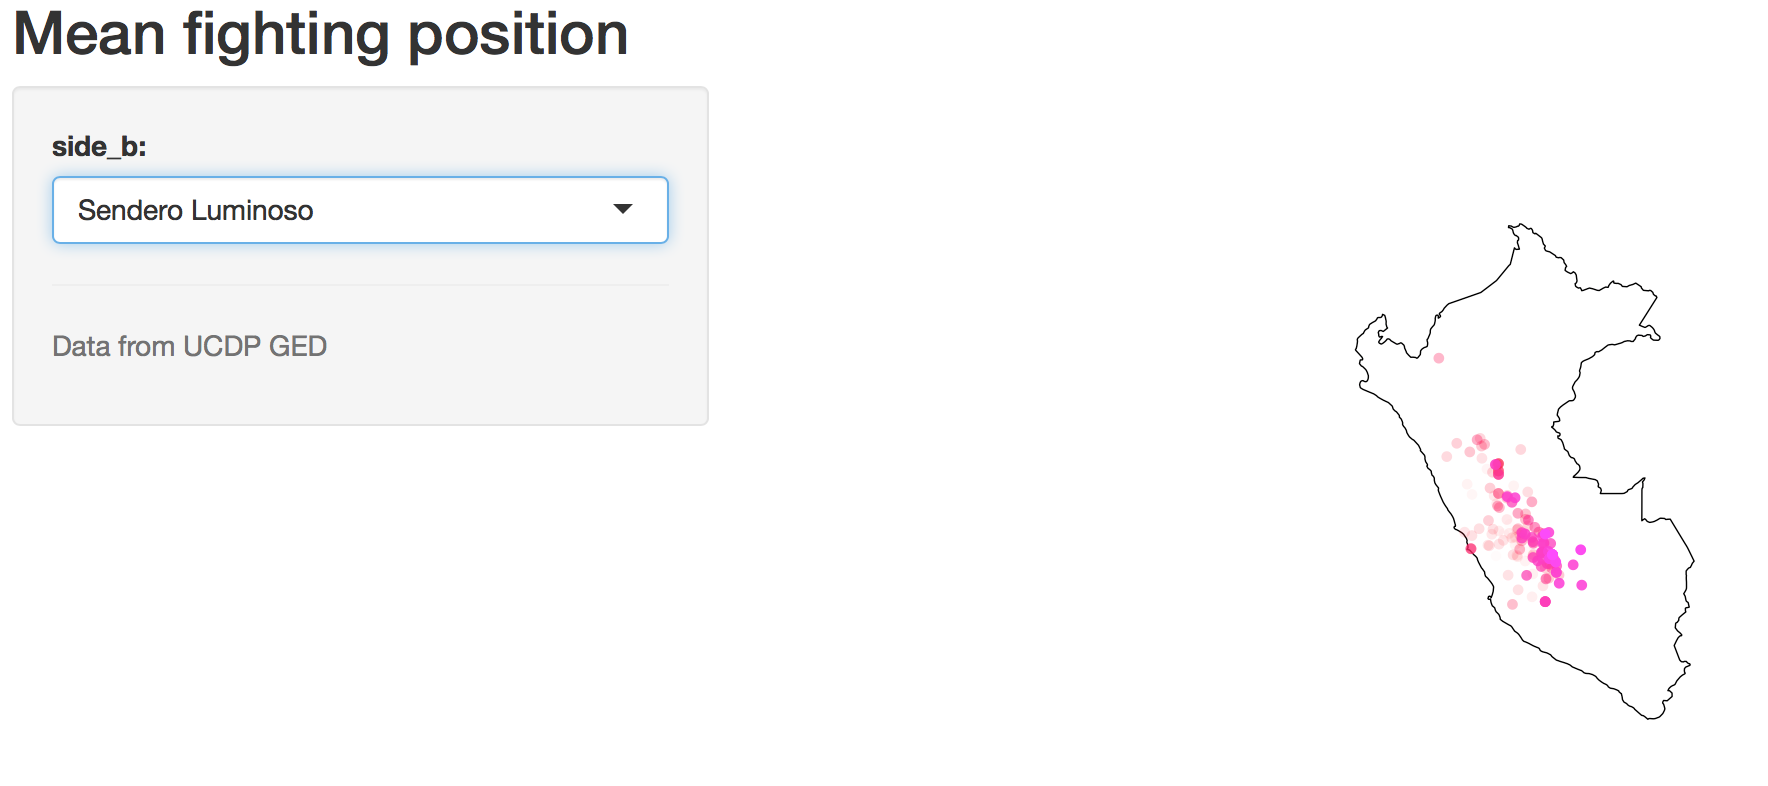
\includegraphics[scale=0.3]{peru_1.png}\\
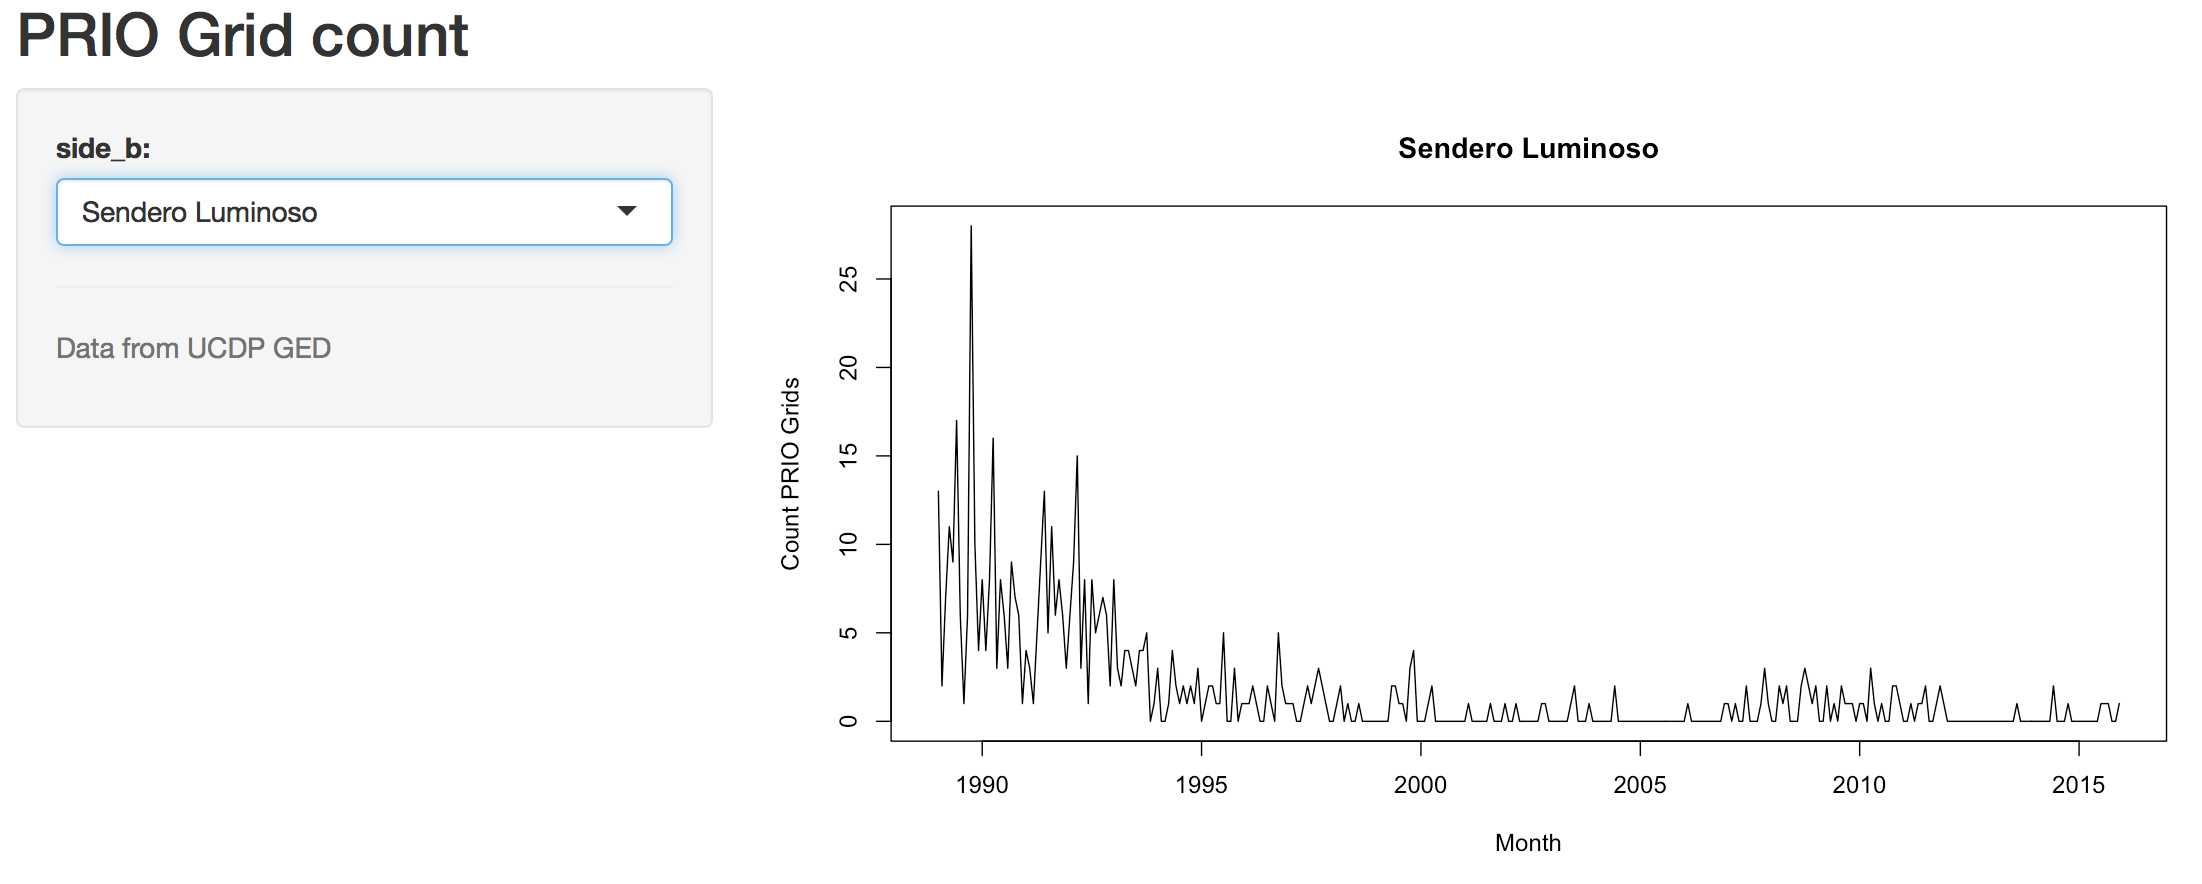
\includegraphics[scale=0.3]{peru_2.png}\\
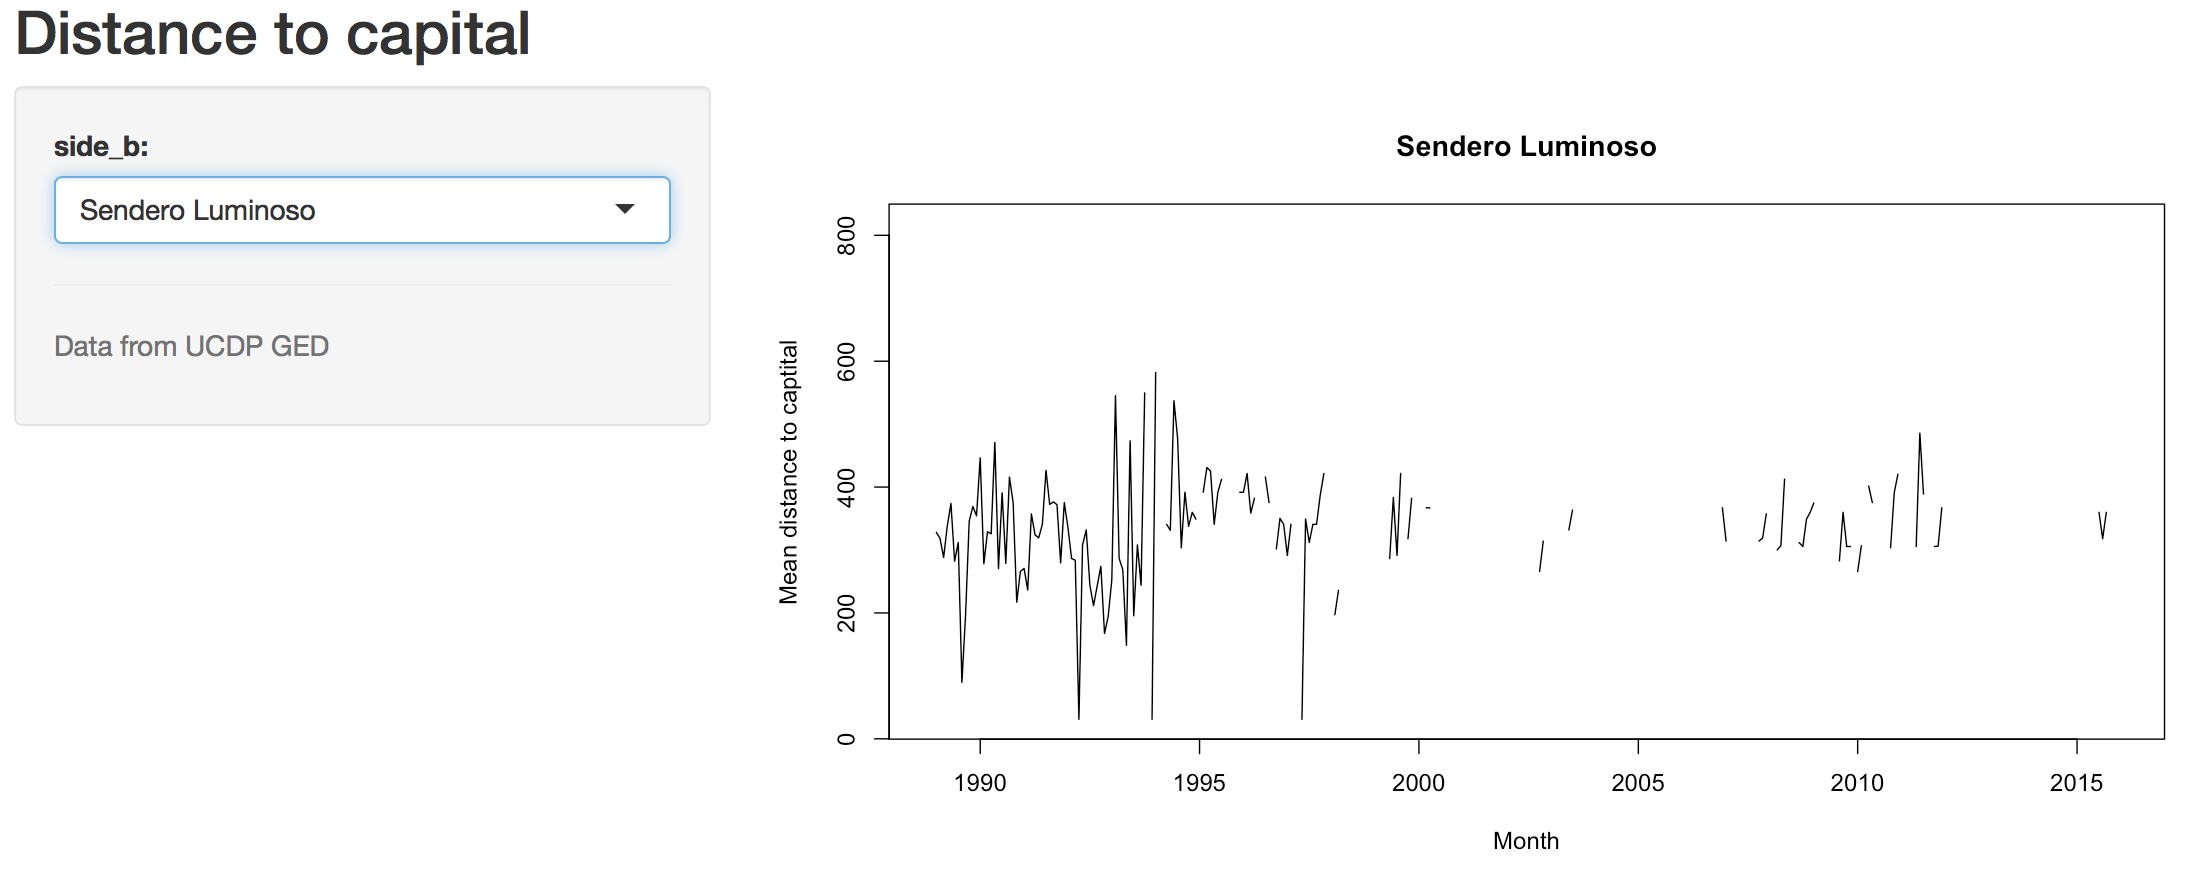
\includegraphics[scale=0.3]{peru_3.png}
\caption{Shiny interface to explore RebelTrack data. Users can choose a specific rebel organization and the respective measurement. Examples provided for Sendero Luminoso in Peru. Top panel: Mean fighting position of rebel organizations, where darker dots represent more recent monthly mean fighting positions. Middle panel: Number of PRIO-grids that are affected by rebel-government fighting in a particular month. Bottom panel: Mean distance of fighting events to the capital.}
\end{figure}


\section{RebelTrack: Measuring actor characteristics and configurations}
In this paper we introduce RebelTrack, which consists of a set of functions to measure rebel behavior, characteristics, and configurations. Using mainly data from the UCDP GED dataset in combination with PRIO grid data, RebelTrack establishes an open-development platform to generate theory and data-driven information on rebel organizations. RebelTrack will be delivered as an R package with an open access Github platform for further development and improvement of existing indicators. The RebelTack package with be updated yearly, with beta versions running on Github for users to access the latest indicators. RebelCast will also develop user requested measures that will included in the annual and beta releases. Data generation and data provision comply with the Data Access and Research Transparency (DA-RT) initiative, which enables researchers using RebelTrack to submit their work to the leading journals in political science and beyond. This includes the provision of a detailed codebook, download date of original data, version number of original data, complete code, and the original data. We hope that this will facilitate the use and development of RebelTrack. 



\subsection{RebelTrack version 1.0, release early Winter 2017}
The initial version of RebelTrack will focus on behavioral measures or rebel organizations. The original functions of RebelTrack allow users to generate monthly, quarterly, or yearly aggregations, but because of the open-source development, users can easily add functionalities to aggregate information on e.g. the daily, weekly, or even 5-year level. Users can also choose whether variables should be lagged and by how many time units. The option to perform missing data imputation is provided. Currently, we have implemented Amelia \citep{king:etal:2001} and a semi-parametric copula approach \citep{hoff:2007}. Some of the variables in the current version 0.8 that will be used in the following RebelCast presentation include:

\subsubsection{\textbf{Mean Capital distance:}} Based on the UCDP GED and PRIO GRID data we provide a function to calculate the mean distance to the country's capital the fighting is taking place in on a monthly, quarterly, or yearly level. The variable can also be provided in monthly, quarterly, or yearly changes.
\subsubsection{\textbf{Min Capital distance:}} Based on the UCDP GED and PRIO GRID data we provide a function to calculate the minimum distance to the country's capital the fighting is taking place in on a monthly, quarterly, or yearly level. The variable can also be provided in monthly, quarterly, or yearly changes.
\subsubsection{\textbf{Max Capital distance:}} Based on the UCDP GED and PRIO GRID data we provide a function to calculate minimal distance to the country's capital the fighting is taking place in on a monthly, quarterly, or yearly level. The variable can also be provided in monthly, quarterly, or yearly changes.
\subsubsection{\textbf{Border distance:}} Based on the UCDP GED and PRIO GRID data we provide a function to calculate the mean distance to the country's border the fighting is taking place in on a monthly, quarterly, or yearly level. The variable can also be provided in monthly, quarterly, or yearly changes.
\subsubsection{\textbf{SideB casualties:}} Based on the best estimates in the UCDP GED data we provide a function to calculate the number of casualties on the rebel side in government-rebel fighting in on a monthly, quarterly, or yearly level. The variable can also be provided in monthly, quarterly, or yearly changes.
\subsubsection{\textbf{SideA casualties:}} Based on the best estimates in the UCDP GED data we provide a function to calculate the number of casualties on the government side in government-rebel fighting in on a monthly, quarterly, or yearly level. The variable can also be provided in monthly, quarterly, or yearly changes.
\subsubsection{\textbf{PRIO grids affected:}} Based on the UCDP GED and PRIO GRID data we provide a function to calculate the number of PRIO grids a rebel organization is active in on a monthly, quarterly, or yearly level. The variable can also be provided in monthly, quarterly, or yearly changes.
\subsubsection{\textbf{Transnational fighting count:}} Based on the UCDP GED and PRIO GRID data we provide a function to calculate the number of countries a rebel organization is active in on a monthly, quarterly, or yearly level. The variable can also be provided in monthly, quarterly, or yearly changes. 
\subsubsection{\textbf{Transnational fighting ratio:}} Based on the UCDP GED and PRIO GRID data we provide a function to calculate the ratio of events that take place in the main activity country of a rebel organization on a monthly, quarterly, or yearly level. The variable can also be provided in monthly, quarterly, or yearly changes.
\subsubsection{\textbf{Resource variables (Diamonds, Drugs, Gold, Oil):}} Based on the UCDP GED and PRIO GRID data we provide a function to calculate the ratio of rebel events that takes place in resource rich areas on a monthly, quarterly, or yearly level. The variable can also be provided in monthly, quarterly, or yearly changes.
\subsubsection{\textbf{Terrain variables):}} Based on the UCDP GED and PRIO GRID  data we provide a function to calculate the ratio of rebel events that takes place urban, mountainous, forrest, and other terrain types on a monthly, quarterly, or yearly level. The variable can also be provided in monthly, quarterly, or yearly changes.





\subsection{RebelTrack version 1.1, release late Winter 2017}
The release of version 1.1. focuses on dependencies and configurations of rebel organizations. It provides information on rebel organizations that are either fighting in the same conflict, the same country, or simply in the same area (distance). Previous research demonstrates that these dependencies should impact on rebel organization duration and the escalation of violence. We provide a set of functions that allow users to create spatially-lagged variables. For example, for rebel organization A, we can calculate how close connected (through distance, conflict ID, or country ID) rebel organizations are to the capital. In the main spatial lag function, users can also define monthly, quarterly, or yearly lags. This gives users full flexibility to create spatio-temporal variables. Users can also contribute connectivity matrices to the github account which will be included in beta and yearly updates of the RebelTrack package.

\subsection{RebelTrack version 1.2, release early Spring 2018}
There are multiple datasets that have collected static and time-varying information on rebel organizations. RebelTrack version 1.2 merges available information, e.g. conflict outcomes \citep{kreutz10}, legal political wings \citep{cunningham09}, or ethnic connections \citep{jwnm:2012}. At this stage we also integrate information on the governments that are fighting the rebel organizations. Characteristics of governments not only influence to duration and escalation of conflict, but they are also likely to interact with characteristics and behavior of the rebel organization. This also relates to potential external support or third party interventions opposing active rebel organizations.


\begin{table}
\caption{Mean AUC scores (across 10 test sets) for all individual models and the ensemble. Higher scores represent models with a better trade-off between and performance of sensitivity and specificity.}
\begin{tabular}{lll}
Method & ROC \\ \hline
 Logit & 0.6587\\
 RF & 0.8122\\
 WSRF & 0.8113\\
 Adaboost & 0.7935\\
 GBM & 0.8536\\
 SVMRadial & 0.5731 \\
 KKNN & 0.5649\\
 NNET & 0.5698\\ \hline
 Ensemble & 0.8189\\
\end{tabular}
\label{tab:roc_models}
\end{table}

\subsection{RebelTrack version 1.3, release late Spring 2018}
Version 1.3 links information from several event datasets \citep{BoscheeElizabethLautenschlagerJenniferOBrien2015,phoenix} by spatial information and name of actors. This relies on similar functionalities that are provided in R packages such as meltt and geomerge. However, merging is optimized for actors present in UCDP GED.  



\section{RebelCast: Predicting rebel organizations durations}
We implement statistical learning approaches to predict the duration of fighting $Y$ in civil wars. Later versions of RebelCast will also include the prediction of escalation and termination type. In order to predict $Y$, we usually have a set of predictors, $X_{1},X_{2},\hdots,X_{p}$ to estimate $Y=f(X)+\epsilon$. Statistical learning approaches stress the estimation of $f$ for prediction and inference. Thus, instead of making assumptions about the functional form of $f$, for example in parametric models, statistical learning approach allow non-linear and non-parametric forms of $f$. When identifying $f$ most statistical learning techniques leverage cross-validation strategies. Our prediction problem is set in a duration context or more specifically in a binary time series cross section format \citet{beck98,carter10}. This means our cross-validation strategy needs to account for time dependent processes as outlined in \citet{cgnm}, who recommend to learn the time-dependency of events by sampling group-wise (in our case baed on rebel organization ID). In the context of binary time series cross section data we are also faced with severe class imbalances which we deal by upsampling as recommended by \citet{Muchlinski01012016} in the context of civil war.

\begin{figure}
\centering
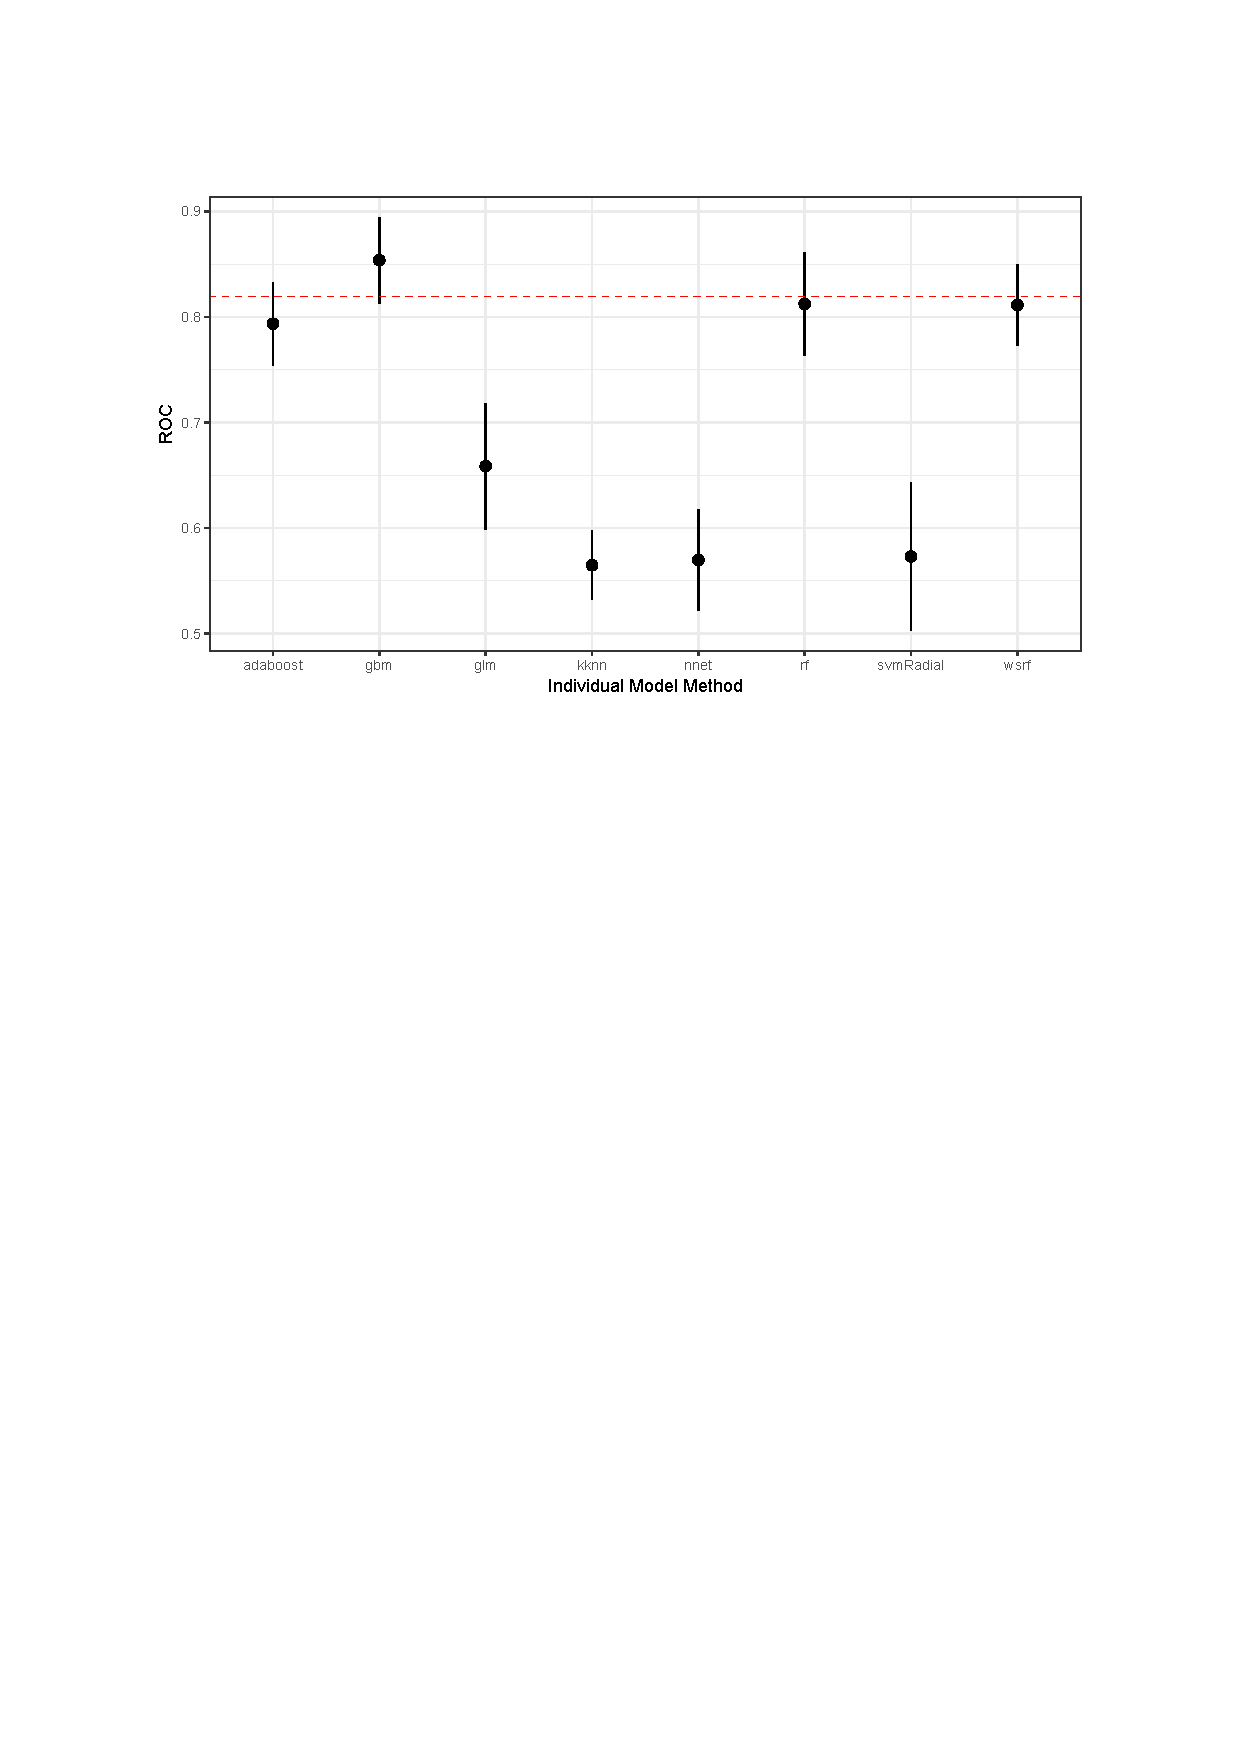
\includegraphics[scale=0.8]{roc_models.pdf}
\caption{Area under the Curve for all eight statistical learning methods that are included in the ensemble model. Red dotted line represents the average ensemble AUC.}
\label{roc_models}
\end{figure}

Our forecasting framework leverages the heterogenous predictive performance of multiple statistical learning tools through an ensemble model. Ensemble methods have been introduced to political science by \citet{montgomery:2012}, but they originate in weather forecasting and stock market predictions. In our ensemble model, we include eight statistical learning tools utilizing the caret package for cross-validation:
\begin{itemize}
\item{Logit: Standard logistic regression model implemented in the R stats package.}
\item{Random Forest: Classification algorithm based on tree classification. Implemented in the R package randomForest.}
\item{Weighted Subspace Random Forest for Classification: Implemented in the R package wsrf. This algorithm optimizes the selection of feature subspaces. Instead of randomly selecting variables to build random forest models, this model excludes non relevant features in the sampling process.}
\item{AdaBoost: This algorithm was developed by Freund and Shapire, 1996. It leverages boosting to increase accuracy and is implemented in the R package fastAdaboost.}
\item{gbm: Generalized Boosted Regression Modeling, which extends the Freund and Shapire, 1996 algorithm. This is implemented in the R package gbm.}
\item{svmRadial: Support Vector Machine implemented in the R kernlab package.}
\item{knn: K-neareast neighbour}: Units are classified according to their k-nearest neighbors is a particular feature space using the class package in R.
\item{nnet: Neural network algorithm implemented in the R package nnet. (See also \citet{Schrodt01101991} for previous neural network approaches in conflict studies.)}
\end{itemize}

In the following models we predict the end of conflict on a quarterly level with the variables described in section 4.1 lagged by one quarter. Our data includes 278 rebel organizations observed in 9377 quarters. In the data, we see 323 fighting episodes that end within the observation period. This number is greater than the number of rebel organizations as each organization can experience multiple spells. As outlined further above we implement a 10-fold cross-validation that ensures that spells are not distributed across different folds. Cross-validation techniques require independence between the training and test set, which is by definition violated in the context of duration models if spells are split into different folds.


\begin{figure}
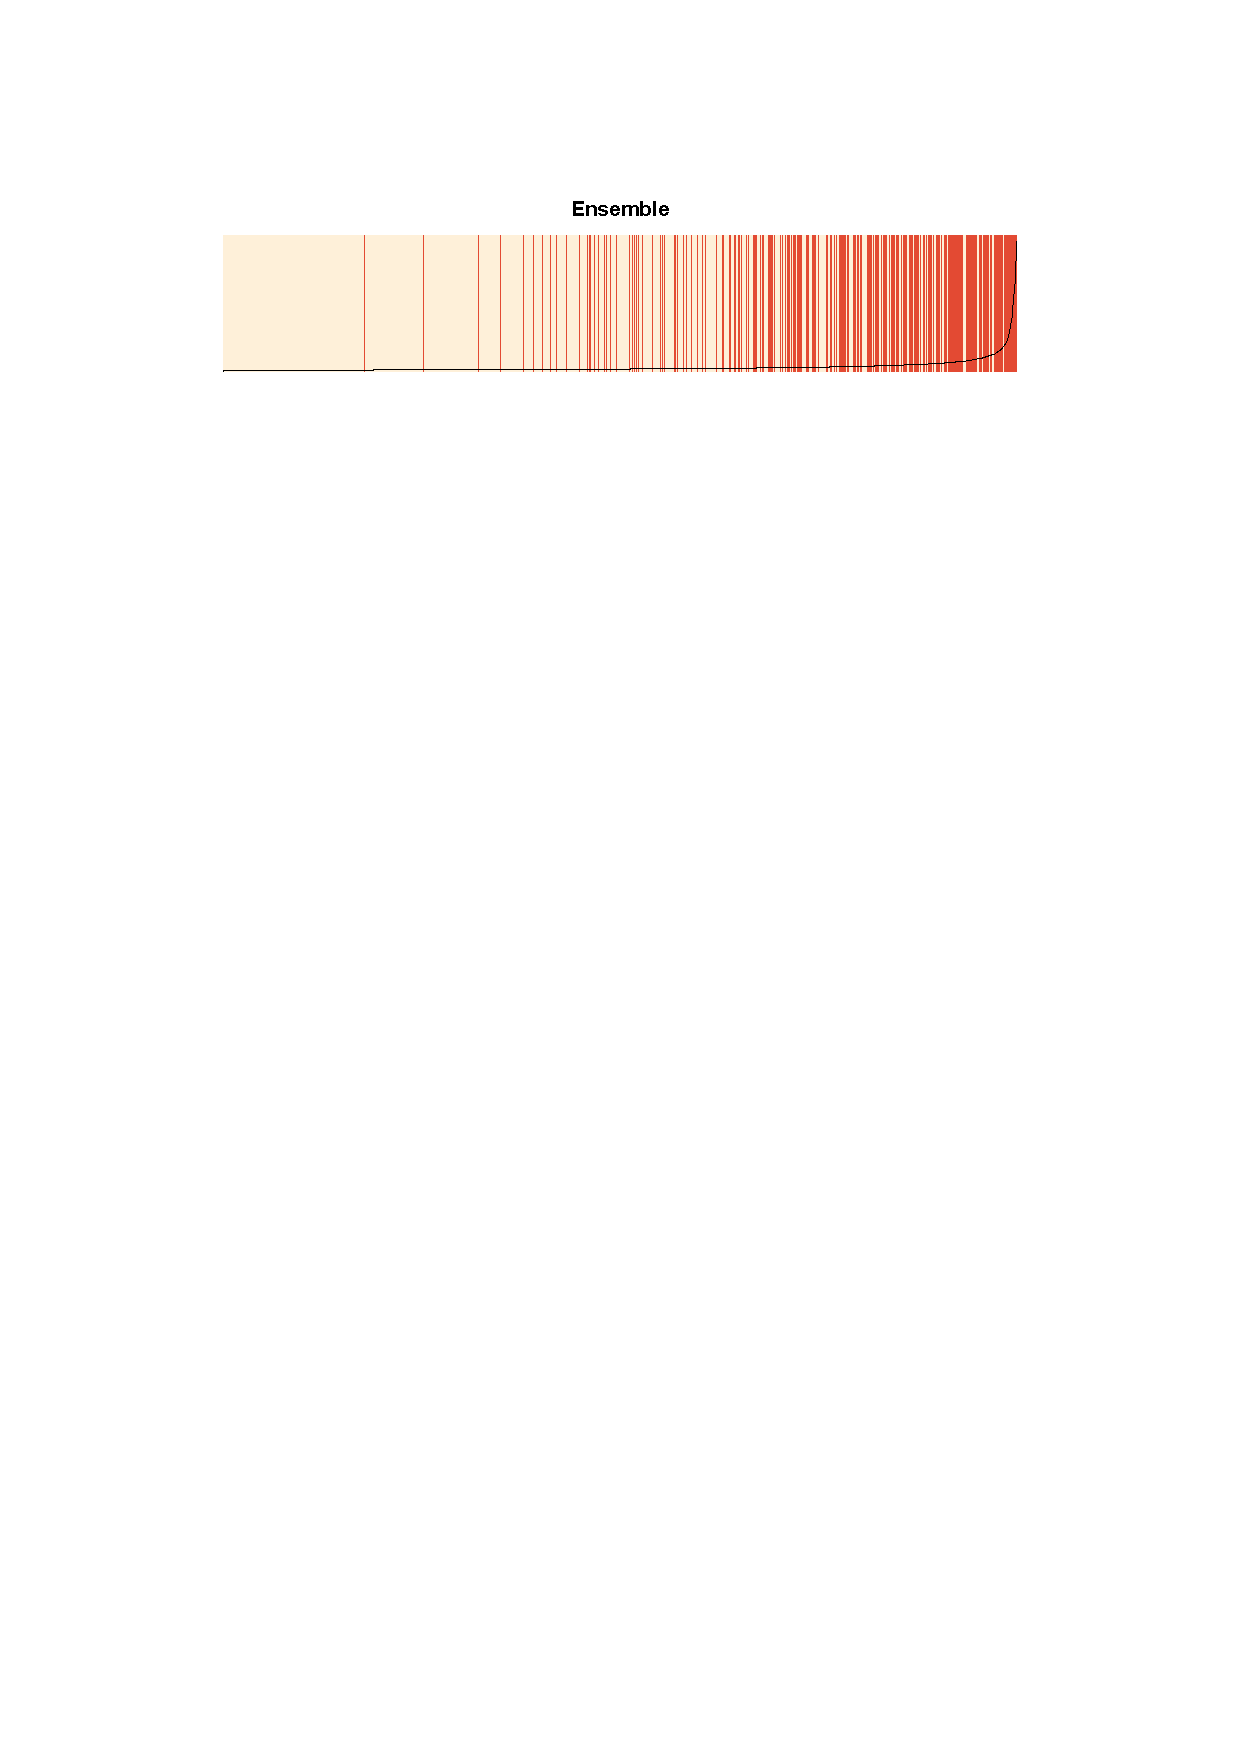
\includegraphics[scale=0.8]{sep_ensemble.pdf}
\label{fig:sep}
\caption{Separationplot from ensemble model ranking observed termination quarters (red) and observed continuation quarters (white) according to their predicted probability from left (low values) to righting (high values) }
\end{figure}

\subsection{Results}
Turning the prediction results, we report test set performance for individual models and the ensemble. First, we calculate the Area under the Curve (AUC) for all eight statistical learning methods that are included in the ensemble. Higher values imply models that have a better trade-off between sensitivity (True-positives) and specificity (True-negatives). In this regard, tree-based methods and related boosting algorithms are outperforming all other approaches. Table~\ref{tab:roc_models} provides the mean AUC score for all individual models and the ensemble, while Figure~\ref{roc_models} also provides insights about the variation of the AUC across all 10 folds. While the GBM has the highest average score (Table~\ref{tab:roc_models}), the ensemble has a lower variation in AUC across the 10-folds. 


\begin{figure}
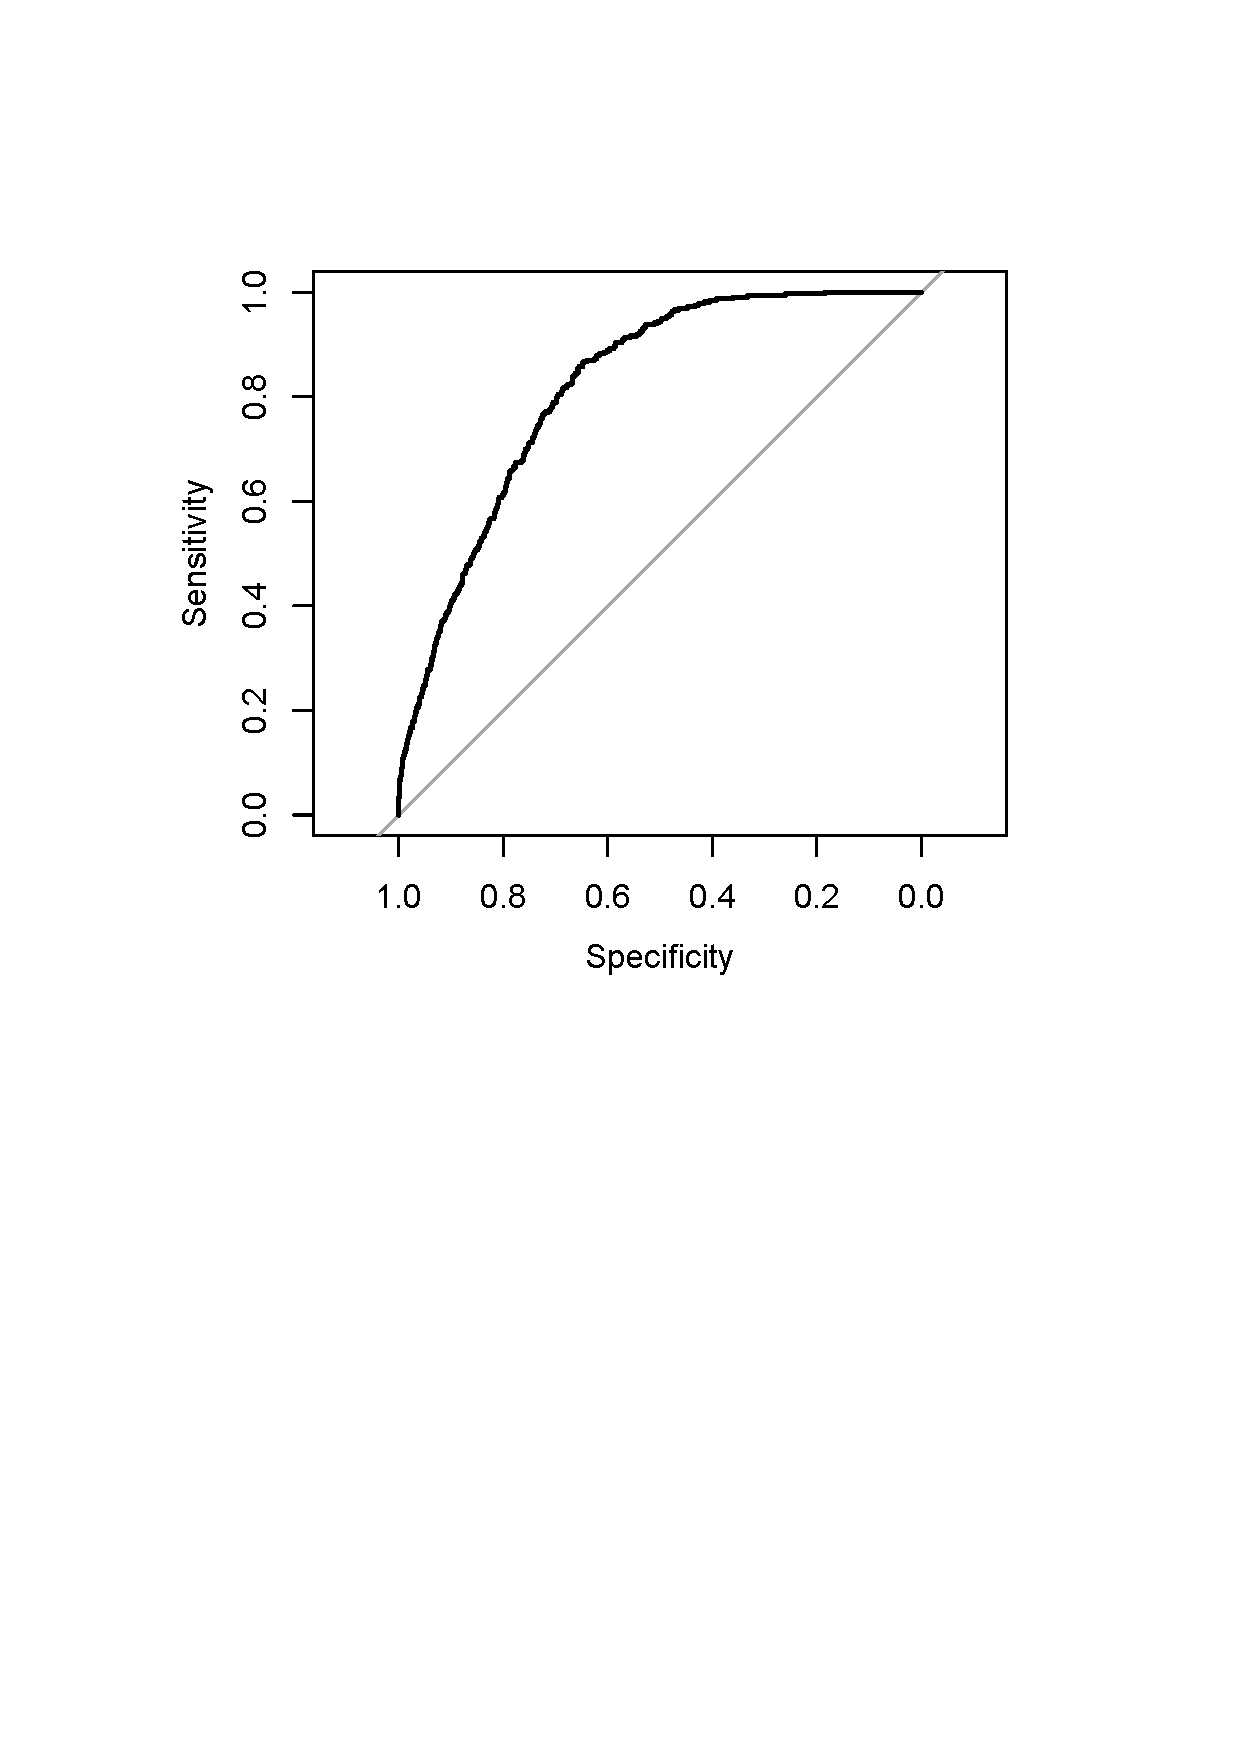
\includegraphics[scale=0.5]{roc_ensemble.pdf}
\label{fig:roc}
\caption{ROC plot showing the tradeoff between sensitivity and specificity of the ensemble model.}
\end{figure}

Focusing further on the ensemble model, we observe that the model generally performs well in assigning high predicted probabilities to quarters the experience the end of fighting. This can be seen in the separation plot in Figure~\ref{fig:sep}, which ranks observed termination quarters (red) and observed continuation quarters (white) according to their predicted probability from left (low values) to righting (high values). However, Table~\ref{tab:confusion} shows that while specificity is generally high, sensitivity is fairly low. Using a conventional classification cutoff of 0.5, leaves us with a True-Positive rate of less than 10 percent. Using a threshold that accounts for the low baseline event probability, by using the mean predicted probability as a cutoff criterium, the True-Positive rate increases to about 66 percent, but the True negative rate declines to around 65 percent. This trade-off can also be seen in the ROC-plot (Figure~\ref{fig:roc}). An increase in sensitivity is associated with a fairly rapid decrease in specificity. We are currently further refining our down-sampling and up-sampling approach to adjust for our class imbalances and initial results provide promising advances.  




\section{Conclusion}
This paper introduces RebelTrack and RebelCast. RebelTrack generates measures of rebel behavior and characteristics with a particular focus on providing an open source platform for developing these indicators further. While researchers have provided a wide range open-source data, there are less efforts to build community developed software that leverages the existing data. Usually, researchers or research teams focus on the development of their own indicators, but little efforts have been made to pool resources of the research community. RebelTrack is also working on ways to ensure that developers are recognized in the citation of RebelTrack and its indicators. We believe that contributing to larger platforms is hampered by academic incentives to generate visible citations (usually through journal publications). Hence, in RebelTrack and also in RebelCast software contributors can apply to become authors of the yearly update paper (and remain so in the next years until authors decide not be listed). We will provide different authorship that will correspond to the extent to which researchers contribute to the R packages.
\begin{itemize}
\item Contributor: Bug fixes and efficiency gains in existing code
\item Provider: Provision of own indicator or measure
\item Coordinator: Coordinator and system administrators 
\end{itemize}
RebelTrack version 1.0 will be released early Winter 2017 and fully available on Github with visualizations on Shiny. Future versions will account for dependency between actors and the inclusion of further event datasets. 

\begin{table}
\caption{Confusion matrices for ensemble model with different classification thresholds. Left confusion matrix with classification threshold = 0.5. Right confusion matrix with the mean of all predicted probabilities as threshold.}
\begin{tabular}{l|l|l|}
& Pred. = 0 & Pred. = 1\\  \hline
Obs. = 0 &  9032  &  22\\
Obs. = 1 & 303 &  20\\ \\ 
\multicolumn{3}{c}{\emph{(A): Classification threshold=0.5 }} \\
\end{tabular}
\begin{tabular}{l|l|l|}
& Pred. = 0 & Pred. = 1\\  \hline
Obs. = 0 &  7014  & 2040\\
Obs. = 1 & 105 &  218\\ \\
\multicolumn{3}{c}{\emph{(B): Classification threshold=Mean }} \\
\end{tabular}
\label{tab:confusion}
\end{table}


\bibliographystyle{apsr}
\bibliography{Nils_Lit2.bib}
\end{document}